\chapter{Related Algorithms} \label{chap:rl}


This chapter will provide deeper introductions into the algorithms discussed in Chapter \ref{chap:intro}.
Section \ref{chap:rl:nn} will introduce neural networks and deep learning in more detail.
Section \ref{chap:rl:tree} will introduce decision trees and random forests, demonstrating a diagram of the tree structure.
Finally Section \ref{chap:rl:lr} will introduce logistic regression.

\section{Neural Networks} \label{chap:rl:nn}

Neural networks are one of the more public-facing machine learning technologies today. They get their name from the structural design of the models, which are inspired by neurons in the brain. Figure \ref{fig:rl:nn} demonstrates what the structure of a basic neural network would look like. Neural networks are organized in layers, where each layer has a different number of nodes ($n$, $m$, and $k$ in Figure \ref{fig:rl:nn}).

\begin{figure}[ht]
    \centering
    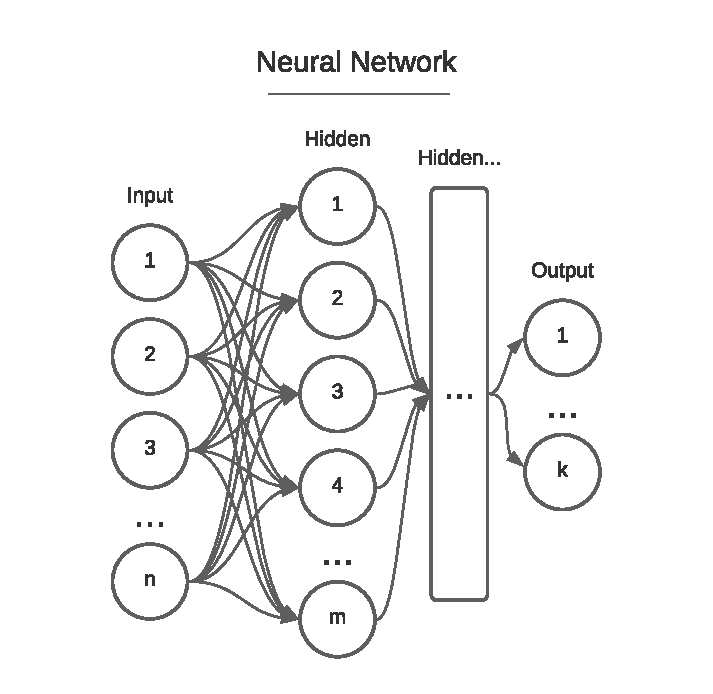
\includegraphics[width=0.8 \textwidth]{Figures/Neural-Network.pdf}
    \caption{An example diagram of basic neural network structure.}
    \label{fig:rl:nn}
\end{figure}

As noted in Chapter \ref{chap:intro}, deep learning techniques based on neural networks \cite{deepmind2020go} \cite{deepmind2020alphafold2} have been widely praised and covered in the media. Deep learning is not practical for use in this project as the size of the data set is too small (Chapter \ref{chap:data}). 

Smaller neural networks can be employed on the DI data.
However, even smaller networks can be hard to interpret, as seen in Figure \ref{fig:rl:nn} the nodes of a neural network are all deeply interconnected. This interconnection is powerful in that it enables the network to create complicated features based on the data during training. These complicated features are double-edged, because they can allow for higher classification performance, but can make it nearly impossible for a human to determine how a classification decision was made. In the simple case of a network with one or two layers and a reasonable number of nodes, it is possible to inspect the network and determine how classifications are made. However, as the number of layers and nodes increases, this power is lost.
Techniques, such as LIME \cite{ribeiro2016lime} \cite{vanberlo2020interpretable} \cite{lundberg2017shap}, have been proposed as a tool that helps overcome the interpretability issue. However, this technique and others like it only help explain why a neural network-based classifier made the classifications it did, they do not help interpret the inner workings of the network itself. 



\section{Decision Trees and Random Forests} \label{chap:rl:tree}
Decision (and regression) trees are another popular tool for creating interpretable models \cite{friedman2001greedy} \cite{chen2016xgboost} \cite{chan2017evidence} \cite{kube2019allocating}. Decision trees start from a single root proposition, such as "Will become chronic?", and iteratively create divisions until the root proposition can be answered with some given degree of certainty. Figure \ref{fig:example-decision-tree} demonstrates the structure of a decision tree. This tree structure makes models immediately interpretable, either by presenting the tree or breaking the tree down into rules of the form "Will become chronic if feature A and feature B". This transparency fades when the tree becomes very large. However, this is usually not an issue as large trees suffer from over-fitting. Over-fitting is the result of a machine learning system that learns patterns in a training population that do not extend to the broader population. This results in poor real world performance and makes over-fitting something to be avoided. Decision trees also suffer from the issue of feature ordering. Tree models are fit by "growing" the tree downwards, meaning the order of feature evaluation is fixed during growth, which can result in a sub-optimal tree structure.
Random forests are a method \cite{toros2019early} that overcome this problem by building an ensemble of decision trees. Random forests make a classification decision by taking a vote of confidence from all trees in the forest, this also helps alleviate the over-fitting problem with decision trees. While random forests are in general a marked improvement over decision trees, they lose the interpretability.

\begin{figure}[ht]
    \centering
    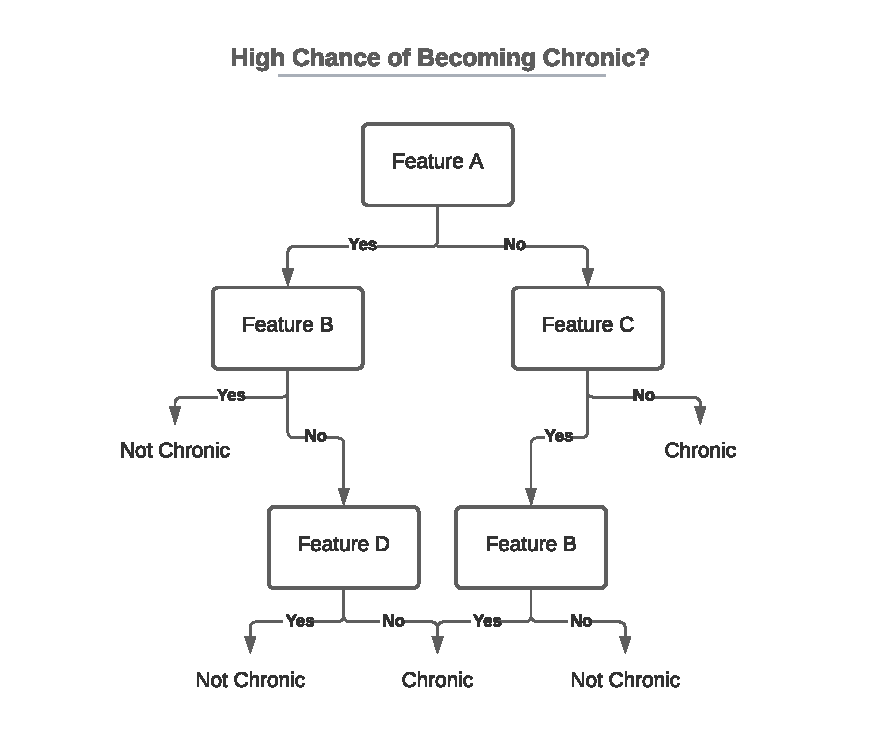
\includegraphics[width=1\textwidth]{Figures/Decision-Tree-Example.pdf}
    \caption{A diagram displaying the structure of a decision tree.}
    \label{fig:example-decision-tree}
\end{figure}

\section{Logistic Regression} \label{chap:rl:lr}
By far the most popular predictive tool in the homeless space is Logistic Regression \cite{hastie2009elements} \cite{king2001LogisticR} \cite{allegheny2019homeless} \cite{hong2018applications} \cite{toros2019early}. Logistic regression is a binary predictor that assumes a combination of feature variables have a linear relationship with the log-odds of an event. Historically, this has been popular because the simple definition lends itself well to interpreting (linear) relationships. Logistic regression is defined as $\log \frac {p}{1-p} = \beta_0 + \beta_1 f_0 + \beta_2 f_1 ...$ where $p$ is the probability of event, $f_n$ are the features based on the data set, and $\beta_n$ are the parameters of the model. The parameter values ($\beta_n$) can be used after training to demonstrate a feature's impact on the classification, leading to a model with a fairly large degree of interpretability.
Logistic regression falls short in two places. First, the model is interpretable for users with the right set of tools, however, the layperson (e.g. front-line shelter staff) is left to trust in parameter values often without the math background to have confidence in the model. Second, the algorithm has a necessary assumption that the data is linearly related, which limits the insights that can be generated. This can be mitigated to a degree by adding new features that are non-linear combinations of existing features, but this method would damage the  interpretability of the model.


% \section{Survival analysis} \label{chap:rl:survival}
% \tdo{Finish the survival analysis section}
% There are also similar algorithms used for regression. Notably in this space is Cox proportional hazards regression \cite{greer2016targeting} \cite{Kim2009UnstableHA}, which is used to calculate some risk value corresponding to the likelihood of a client entering/re-entering homelessness. This technique is especially popular in the homeless space, as it provides an approximate "time to event" rather than a binary flag. 

